\chapter{Kinematics}
As we already know the robot can be represented as a kinematic chain of links and connected by revolute joints. In this chapter the forward kinematics for this robotic manipulator is calculated and a method for solving the inverse kinematics is proposed. 

\section{Forward Kinematics}
The forward kinematics states the relationship between the end effector and the individual joints. Or as \cite{Siciliano} says it: The motion of the structure is obtained by composition of the elementary motions of each link with respect to the previous one. An easy way to get the forward kinematics is to use the Denavit-Hartenberg(DH) convention. \cite{spong} states that each homogeneous transformation $A_i$ is represented as a product of four basic transformations: 

$$
A_i = \text{Rot}_{z,\theta_i}\text{Trans}_{z,d_i}\text{Trans}_{x,a_i}\text{Rot}_{x,\alpha_i}=
    \begin{bmatrix}
        c_{\theta_i} & -s_{\theta_i}c_{\alpha_i} & s_{\theta_i}s_{\alpha_i} & a_ic_{\theta_i}\\
        s_{\theta_i} & c_{\theta_i}c_{\alpha_i} & -c_{\theta_i}s_{\alpha_i} & a_is_{\theta_i}\\
        0 & s_{\alpha_i} & c_{\alpha_i} &d_i\\
        0 & 0 & 0 & 1
    \end{bmatrix}
$$

where $c_{\theta_i} = \cos{(\theta_i)}$ and $s_{\theta_i} = \sin{(\theta_i)}$, and the same for $\alpha$. $A_i$ is a transformation matrix which states the transformation between link number $i$ and link number $i-1$. This means that it is possilbe to get the transformation from the robot base to the end effector by multiplying each transformation matrix:
\begin{align*}
    T^i_j = A_{i+1}A_{i+2}...A_j, \quad i<j
\end{align*}
 $T^i_j$ states the transformation between each link and it has the form
 \begin{align*}
      T^i_j = 
      \begin{bmatrix}
          R^i_j & o^i_j\\
          0&1
      \end{bmatrix}, \quad i<j
 \end{align*}
 where $R^i_j = R^i_{i+1}R...R^{j-1}_j$ which is the orientation of $o_jx_jy_jz_j$ relative to $o_ix_iy_iz_i$. $o^i_j$ is the coordinate vector which can be written as $o^i_j = o^i_{j-1}+R^{i}_{j-1}o^{j-1}_j$. This is useful when finding the Jacobian of the robot and to verify that the end effector is at the wanted position and has the wanted orientation in the Cartesian world frame. When finding the DH-parameters they have to satisfy the two following properties (\cite{spong}).
 \begin{itemize}
     \item The axis $x_n$ is perpendicular to the axis $z_{n-1}$
     \item The axis $x_n$ intersects the axis $z_{n-1}$
 \end{itemize}

In \figref{fig:dhf} the different axis are set with respect to the DH properties stated above. 

\begin{figure}[htbp]
  \centering
  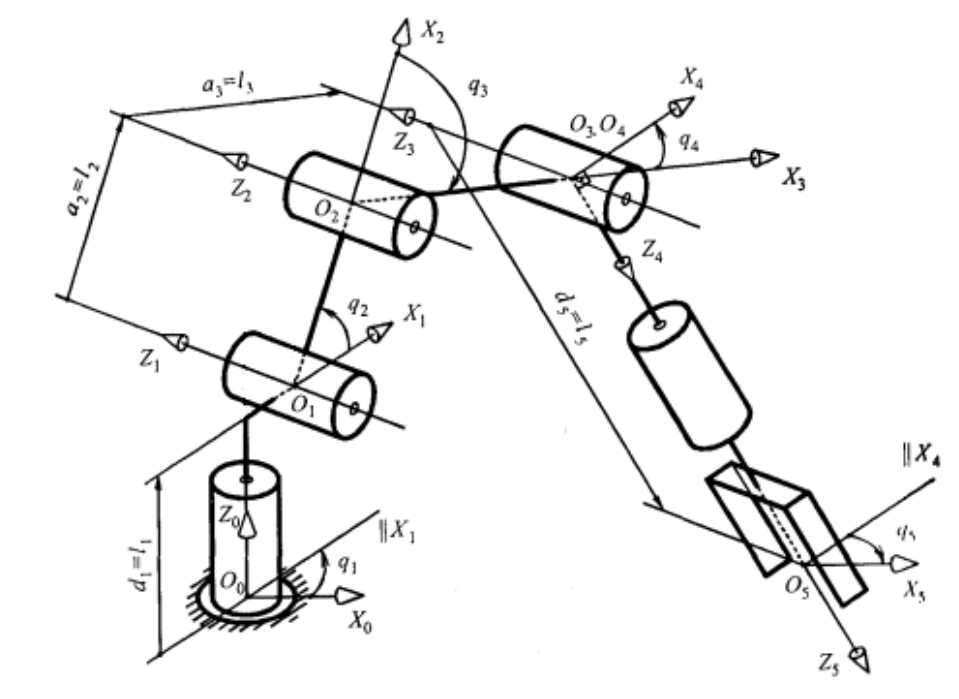
\includegraphics[width=.9\textwidth]{img/DHconv.png}
  \caption{Kinematic scheme of the manipulator. Source \cite{Kinematics}}
  \label{fig:dhf}
\end{figure}

By looking at \figref{fig:dhf} the following DH parameters are found:
\begin{center}
    \begin{tabular}{|c|c|c|c|c|}
         \hline
         Link & $a_i$ & $\alpha_i$ & $d_i$ & $\theta_i$ \\ \hline
         1 & 0 & $-\frac{\pi}{2}$ & $d_1$ & $q_1$ \\
         2 & $a_2$ & 0 & 0 & $q_2$ \\ 
         3 & $a_3$ & 0 & 0 & $q_3$\\
         4 & 0 & $\frac{\pi}{2}$ & 0 & $q_4$\\
         5 & 0 & 0 & $d_5$ & $q_5$\\
         \hline
    \end{tabular}
\end{center}

% d_1 = 0.0506
% a_2 = 0.0506 + 0.0206 + 0.0635 = 0.1347
% a_3 = 0.0506 + 0.0206 = 0.0712
% d_5 = 0.0506 + 0.0206 + 0.0253 + 0.08 = 0.1765

where $d_1 = 0.0506$, $a_2 = 0.1347$, $a_3 = 0.0712$ and $d_5 = 0.1765$ for the model. The real values need to be measured properly since the data sheet of the robot is insufficient and this is just guesstimated values. 
Now it is possible to calculate $A_i$ for each link: 
\begin{align*}
A_1 &= \begin{bmatrix} 
            c_1 & 0 & -s_1 & 0\\
            s_1 & 0 & c_1 & 0\\
            0 & -1 & 0 & d_1\\
            0 & 0 & 0 & 1
        \end{bmatrix},
A_2 = \begin{bmatrix} 
            c_2 & -s_2 & 0 & a_2c_2\\
            s_2 & c_2 & 0 & a_2s_2\\
            0 & 0 & 1 & 0\\
            0 & 0 & 0 & 1
        \end{bmatrix},
A_3 = \begin{bmatrix} 
            c_3 & -s_3 & 0 & a_3c_3\\
            s_3 & c_3 & 0 & a_3s_3\\
            0 & 0 & 1 & 0\\
            0 & 0 & 0 & 1
        \end{bmatrix}\\
A_4 &= \begin{bmatrix} 
            c_4 & 0 & s_4 & 0\\
            s_4 & 0 & -s_4 & 0\\
            0 & 1 & 0 & 0\\
            0 & 0 & 0 & 1
        \end{bmatrix},
A_5 = \begin{bmatrix} 
            c_5 & -s_5 & 0 & 0\\
            s_5 & c_5 & 0 & 0\\
            0 & 0 & 1 & d_5 \\
            0 & 0 & 0 & 1
        \end{bmatrix}
\end{align*}
 and then calculate $T_i^0$:
\begin{subequations}
    \begin{align}
        T_1^0 &= A_1 =
        \begin{bmatrix}\label{eq:T1}
            c_1 & 0 & -s_1 & 0\\
            s_1 & 0 & c_1 & 0\\
            0 & -1 & 0 & d_1\\
            0 & 0 & 0 & 1
        \end{bmatrix}\\
        T_2^0 &= A_1A_2 =
        \begin{bmatrix}\label{eq:T2}
            c_1c_2 & -c_1s_2 & -s_1 & a_2c_1c_2\\
            s_1c_2 & -s_1s_2 & c_1 & a_2s_1c_2\\
            -s_2 & -c_2 & 0 & d_1 - a_2s_2\\
            0 & 0 & 0 & 1
        \end{bmatrix}\\
        T_3^0 &= A_1A_2A_3=
        \begin{bmatrix}\label{eq:T3}
            c_{23}c_1 & -c_1s_{23} & -s_1 & c_1(a_3c_{23} + a_2c_2)\\
            c_{23}s_1 & -s_1s_{23} & c_1 & s_1(a_3c_{23} + a_2c_2)\\
            -s_{23} & -c_{23} & 0 & d_1 - a_3s_{23}-a_2s_2\\
            0 & 0 & 0 & 1
        \end{bmatrix}\\
        T_4^0 &= A_1A_2A_3A_4=
        \begin{bmatrix}\label{eq:T4}
            c_1c_{234} & -s_1 & c_1s_{234} & c_1(a_3c_{23} + a_2c_2)\\
            s_1c_{234} & c_1 & s_1s_{234} & s_1(a_3c_{23} + a_2c_2)\\
            -s_{234} & 0 & c_{234} & d_1 - a_3s_{23} - a_2s_2\\
            0 & 0 & 0 & 1
        \end{bmatrix}\\
        \begin{split}
            T_5^0 &= A_1A_2A_3A_4A_5\\ &=
            \begin{bmatrix}\label{eq:T5}
                c_1c_{234}c_5 - s_1s5 & -s_1c_5 - c_1c_{234}s_5 & c_1s_{234} & c_1(a_3c_{23} + a_2c_2 + d_5s_{234})\\
                s_1c_{234}c_5 + c_1s_5 & c_1c_5 - s_1c_{234}s_5 & s_1s_{234} & s_1(a_3c_{23} + a_2c_2 + d_5s_{234})\\
                -s_{234}c_5 & s_{234}s_5 & c_{234} & d_1 - a_3s_{23} - a_2s_2 + d_5c_{234}\\
                0 & 0 & 0 & 1
            \end{bmatrix}
        \end{split}
     \end{align}
\end{subequations}
where $s_{ijk} = \sin{(q_i + q_j + q_k)}$ and the same for $c_{ijk}$. 
%The $T_i^0$ matrix can be sectioned into
%\begin{align*}
 %T_i^0 = 
  %  \begin{bmatrix}
   %     \bm{R}(\bm{q}) & \bm{p}(\bm{q})\\
    %    \bm{0}^T & 1
    %\end{bmatrix}    
%\end{align*}

%-----------------------------------------------------------------------------------------
\begin{comment}
\begin{align*}
    T^0_5 &= A_1A_2A_3A_4A_5\\
    &= 
    \begin{bmatrix}
        c_1c_{234}c_5 + s_1s_5 & -c_1c_{234}s_5+s_1c_5 & -c_1s_{234} & c_1(-d_5s_{234} + a_3c_{23} + a_2c_2)\\
        c_1c_{234}c_5 - s_1s_5 & -s_1c_{234}s_5-c_1c_5 & -s_1s_{234} & s_1(-d_5s_{234} + a_3c_{23} + a_2c_2) \\
        -s_{234}c_5 & s_{234}s_5 & -c_{234} &d_1 - a_2s_2 - a_3s_{23} - d_5c_{234}\\
        0 & 0 & 0 & 1\\
    \end{bmatrix}\\
    &=
    \begin{bmatrix}
        \bm{R}(\bm{q}) & \bm{p}(\bm{q})\\
        \bm{0}^T & 1
    \end{bmatrix}
\end{align*}
\end{comment}
%-----------------------------------------------------------------------------------------

\subsection{Direct kinematics}
(Just a smaller representation of the forward kinematics)

\subsection{Jacobian}
As we already know the forward kinematics can be written as:
\begin{align*}
    T(q) = 
    \begin{bmatrix}
        R(q) & p(q)\\
        0 & 1
    \end{bmatrix}
\end{align*}
we want to express the linear velocity $\dot{p}$ and angular velocity $\omega$ as a function of the joint velocities $\dot{q}$. In \cite{Siciliano} the relations is stated as:

\begin{equation}
    \begin{aligned}\label{eq:velo}
        \dot{p} &= J_P(q)\dot{q}\\
        \omega&= J_O(q)\dot{q}
    \end{aligned}
\end{equation}

where $J_O$ with dimensions (3 $\times$ n) is the relation between the joint velocities $\dot{q}$ and the end-effector linear velocity $\dot{p}$, and the (3 $\times$ n) matrix $J_O$ is the relation between the joint velocities $\dot{q}$ and the end-effector angular velocity $\omega$. \eqref{eq:velo} can be written as

\begin{align*}
    v_e = 
    \begin{bmatrix}
        \dot{p} \\ \omega
    \end{bmatrix}
    = J(q)\dot{q}
\end{align*}
where
\begin{align*}
    J = 
    \begin{bmatrix}
        J_P \\ J_O
    \end{bmatrix}
\end{align*}

which is the matrix that \cite{Siciliano} calls the geometric Jacobian. The elements of 
$$
J = 
\begin{bmatrix}
    j_{P1} & & j_{Pn}\\
    &...&\\
    j_{O1} & & j_{On}
\end{bmatrix}
$$
can be calculated in the following way:
\begin{align*}
    \begin{bmatrix}
        j_{Pi}\\j_{Oi}
    \end{bmatrix}
    =
    \begin{cases}
        \begin{bmatrix} z_{i-1}\\ 0 \end{bmatrix} & \text{for a prismatic joint}\\
        \begin{bmatrix} z_{i-1} \times (p_e-p_{i-1}) \\ z_{i-1} \end{bmatrix} & \text{for a revolute joint}
    \end{cases}
\end{align*}

Since our manipulator only has revolute joints, the geometric Jacobian becomes

\begin{align*}
    J(q) = 
    \begin{bmatrix}
        z_0 \times (p_5-p_0) & 
        z_1 \times (p_5-p_1) & 
        z_2 \times (p_5-p_2) & 
        z_3 \times (p_5-p_3) & 
        z_4 \times (p_5-p_4) \\
        z_0 &
        z_1 &
        z_2 &
        z_3 &
        z_4
    \end{bmatrix}
\end{align*}
From when the forward kinematics were calculated each position vector $p_i$ can be directly obtained from the equations \eqref{eq:T1} - \eqref{eq:T5}:



\begin{align*}
    p_0 = \begin{bmatrix} 0 \\ 0 \\ 0 \end{bmatrix}    \quad
    p_1 = \begin{bmatrix} 0 \\ 0 \\ d_1\end{bmatrix}    \quad
    p_2 = \begin{bmatrix} a_2c_1c_2\\ a_2s_1c_2\\ d_1 - a_2s_2\end{bmatrix}   \quad 
    p_3 = \begin{bmatrix} c_1(a_3c_{23} + a_2c_2) \\ s_1(a_3c_{23} + a_2c_2) \\ d_1 - a_3s_{23}-a_2s_2 \end{bmatrix}  \\  
    p_4 = \begin{bmatrix} c_1(a_3c_{23} + a_2c_2) \\ s_1(a_3c_{23} + a_2c_2) \\ d_1 - a_3s_{23}-a_2s_2\end{bmatrix}  \quad  
    p_5 = \begin{bmatrix} c_1(a_3c_{23} + a_2c_2 + d_5s_{234}) \\ s_1(a_3c_{23} + a_2c_2 + d_5s_{234}) \\ d_1 - a_3s_{23} - a_2s_2 + d_5c_{234} \end{bmatrix}    
\end{align*}

The next step is to find $z_{i-1}$. \cite{Siciliano} states that $z_{i-1}$ is given by the third column of the rotation matrix $R_{i-1}^0$. $R_{i-1}^0$ is already given in $T_i^0$, By looking at \eqref{eq:T1} - \eqref{eq:T5} the following values of $z_{i-1}$ is given:
\begin{align*}
    z_0 &= \begin{bmatrix}0\\0\\1\end{bmatrix},
    z_1 = \begin{bmatrix}-s_1\\c_1\\0\end{bmatrix},
    z_2 = \begin{bmatrix}-s_1\\c_1\\0\end{bmatrix},
    z_3 = \begin{bmatrix}-s_1\\c_1\\0\end{bmatrix},
    z_4 = \begin{bmatrix}c_1s_{234}\\s_1s_{234}\\c_{234}\end{bmatrix}
\end{align*}

now we got everything needed to compute the geometric Jacobian and the result is presented below.


\begin{align*}
    J(q) &= \\
    &\begin{bmatrix}
        -s_1(a_3c_{23} + a_2c_{2} + d_5s_{234}) & 
        -c_1(a_3s_{23} + a_2s_{2} - d_5c_{234}) & 
        -c_1(a_3s_{23} - d_5c_{234})            & 
        c_1d_5c_{234}                           & 
        0\\
        c_1(a_3c_{23} + a_2c_{2} + d_5s_{234})  & 
        -s_1(a_3s_{23} + a_2s_{2} - d_5c_{234}) & 
        -s_1(a_3s_{23} - d_5c_{234})            & 
        s_1d_5c_{234}                           & 
        0\\
        0                                       &
        -a_3c_{23}- a_2c_2 - d_5s_{234}         &
        -a_3c_{23} - d_5s_{234}                 &
        -d_5s_{234}                             &
        0\\
        0                                       &
        -s_1                                    &
        -s_1                                    &
        -s_1                                    &
        c_1s_{234}\\
        0                                       &
        c_1&
        c_1&
        c_1&
        s_1s_{234}\\
        1& 0 & 0 & 0 & c_{234}
    \end{bmatrix}
\end{align*}
which has the full rank of $5$. 


\section{Inverse Kinematics(outdated)}
\cite{Siciliano} states that one can use the Jacobian of the system to calculate the inverse kinematics:

\begin{align}\label{eq:algo}
\dot{\bm{e}} = \dot{\bm{x}}_d - \bm{J}_A(\bm{q})\dot{\bm{q}}
\end{align}

In \figref{fig:inverseAlgo} the inverse kinematics algorithm is stated. From the figure one can see that 
$$
\dot{\bm{q}} = \bm{J}_A^{-1}(\bm{q})(\dot{\bm{x}}_d + \bm{K}e)
$$
where K is a positive definite diagonal matrix which makes the resulting system \eqref{eq:algo} into the linear system
\begin{align*}
    \dot{\bm{e}} + \bm{K}e = \bm{0}
\end{align*}


\begin{figure}[htbp]
  \centering
  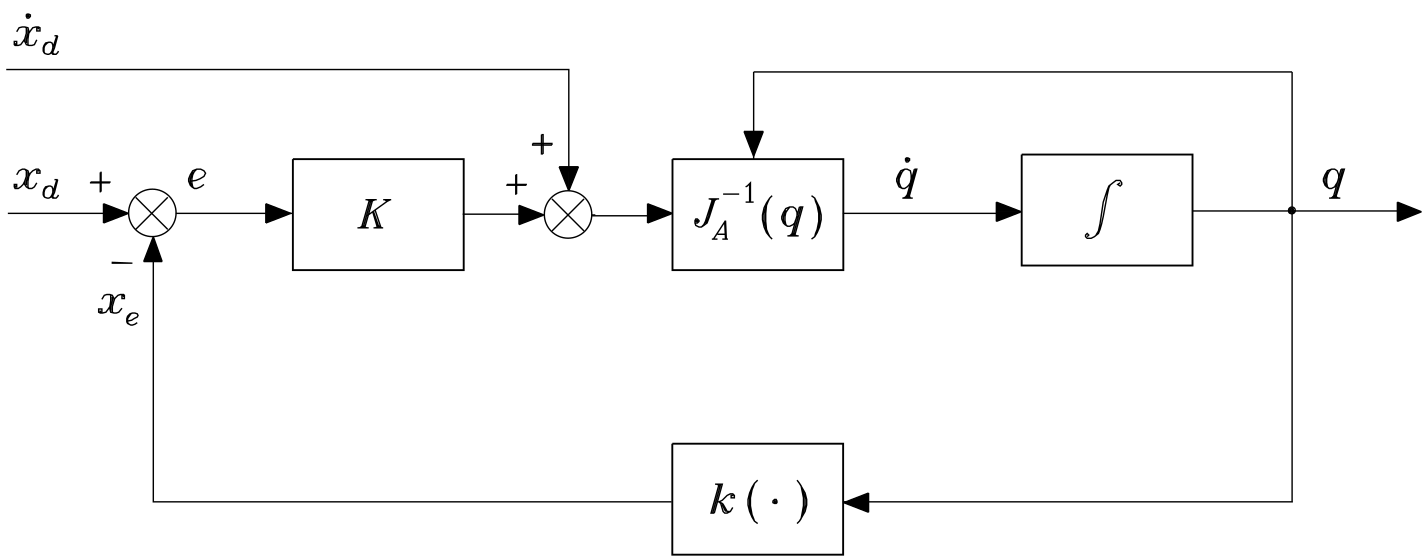
\includegraphics[width=.9\textwidth]{img/inverseKin.png}
  \caption{Inverse kinematics algotihm with Jacobian inverse. Source \cite{Siciliano}.}
  \label{fig:inverseAlgo}
\end{figure}

\subsubsection*{Analytical Jacobian}
To use the algorithm in \figref{fig:inverseAlgo} the analytical Jacobian is needed. In \cite{Siciliano} the following relationship is given
\begin{align*}
    \bm{J}_A =
    \begin{bmatrix}
        \bm{I} & \bm{0}\\ 0 & \bm{T}^{-1}(\bm{\phi_e})
    \end{bmatrix}
    \bm{J}(\bm{q})
\end{align*}

where $\bm{\phi_e} = [\phi,\theta,\psi]^T$ is the orientation of the end-effector frame relative to the base frame given by the Euler angles ZYZ. From \eqref{eq:T5} the rotation matrix from the base frame to end-effector is
\begin{align*}
    \bm{R}_5^0 &= 
    \begin{bmatrix}
        r_{11} & r_{12} & r_{13}\\
        r_{21} & r_{22} & r_{23}\\
        r_{31} & r_{32} & r_{33}
    \end{bmatrix}
    =
    \begin{bmatrix}
        c_1c_{234}c_5 - s_1s_5 & -s_1c_5 - c_1c_{234}s_5 & c_1s_{234}\\
        s_1c_{234}c_5 + c_1s_5 & c_1c_5 - s_1c_{234}s_5 & s_1s_{234}\\
        -s_{234}c_5 & s_{234}s_5 & c_{234} 
    \end{bmatrix}
\end{align*}

The ZYZ Euler angles are then


\begin{align*}
    \phi &= atan2(r_{21},r_{11}) = atan2(s_1c_{234}c_5 + c_1s_5,c_1c_{234}c_5 - s_1s_5)\\
    \theta &= atan2\left(-r_{31},-\sqrt{r_{32}^2+r_{33}^2}\right) = atan2\left(s_{234}c_5,-\sqrt{s_{234}s_5^2+c_{234}^2}\right)\\
    \psi &= atan2(r_{32},r_{33}) = atan2(s_{234}s_5,c_{234})
\end{align*}

The angular velocity $\bm{\omega}_e$ and $\bm{T}(\bm{\alpha})$ is given as

\begin{align*}
    \bm{\omega} = 
    \begin{bmatrix}
        0 & -s_\phi & c_\phi s_\theta\\
        0 & c_\phi & s_\phi s_\theta\\
        1 & 0 & c_\theta
    \end{bmatrix}
    \begin{bmatrix}
        \dot{\phi}\\\dot{\theta}\\\dot{\psi}
    \end{bmatrix}
    =
    \bm{T}(\bm{\phi}_e)\dot{\bm{\phi}}_e
\end{align*}
The determinant of $\bm{T}$ is $-s_\theta$ which means that one cannot invert for $\theta = 0,\pi$. This singularity is also the singularity of the geometric Jacobian. 







%\begin{comment}
If the desired position is $p$ and the desired orientation is $R$. Then in \cite{Kinematics}, the inverse kinematics are given as: 

\begin{align*}
    q_1 &= \tan^{-1}{\left(\frac{p_y}{p_x}\right)}\\
    q_2 &= atan2\left( a(a_2+a_3c_3) - ba_3s_3, aa_3s_3 + b(a_2+a_3c_3) \right)\\%atan2
    q_3 &= \cos^{-1}{\left(\frac{a^2+b^2-a^2_2-a^2_3}{2a_2a_3}\right)}\\
    q_4 &= q_{234} - q_2 - q_3\\
    q_5 &= c_{234}q_1-2atan(R_{21},R_{11})
\end{align*}

where $a = d_1 - d_5c_{234}-p_z$, $b = p_xc_1 + p_ys_1+d_5s_{234}$ and $-\frac{\pi}{2}<q_1 < \frac{\pi}{2}$. $q_{234} = atan2\left(\frac{p_x}{c_1p_x+s_1p_y})\right)$

%\cite{Siciliano}
%\end{comment}


\section{Inverse Kinematics}
\section{Motion planning}